% Generated by paper/gen.py from paper/data. Do not edit.
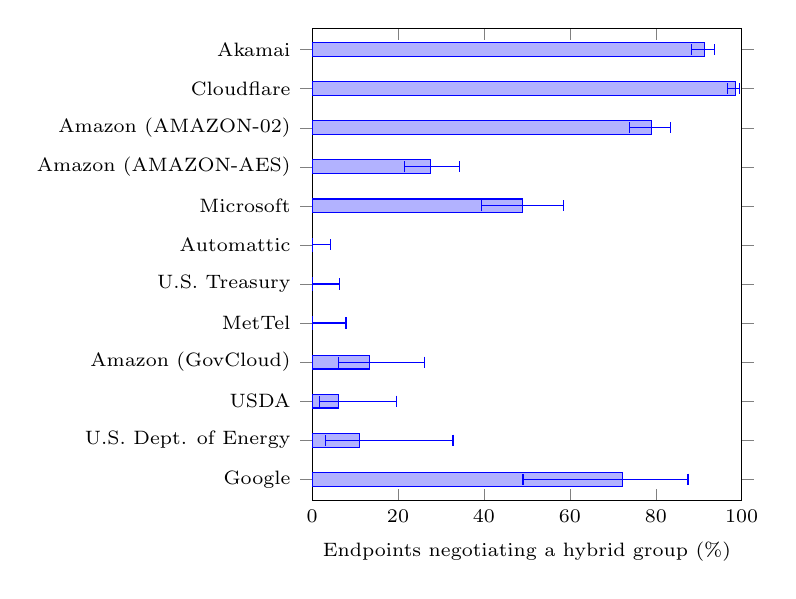
\begin{tikzpicture}
\begin{axis}[
  xbar, xmin=0, xmax=100, scale only axis, width=0.45\linewidth, height=6cm,
  xlabel={Endpoints negotiating a hybrid group (\%)},
  ytick={0,...,11},
  yticklabels={{Google},{U.S. Dept. of Energy},{USDA},{Amazon (GovCloud)},{MetTel},{U.S. Treasury},{Automattic},{Microsoft},{Amazon (AMAZON-AES)},{Amazon (AMAZON-02)},{Cloudflare},{Akamai}},
  y tick label style={font=\scriptsize}, x tick label style={font=\scriptsize},
  label style={font=\scriptsize}, bar width=5pt, enlarge y limits=0.05,
]
\addplot+[error bars/.cd, x dir=both, x explicit] coordinates {
  (72.2,0) += (15.3,0) -= (23.1,0)
  (11.1,1) += (21.7,0) -= (8.0,0)
  (6.1,2) += (13.5,0) -= (4.4,0)
  (13.3,3) += (12.8,0) -= (7.1,0)
  (0.0,4) += (7.9,0) -= (0.0,0)
  (0.0,5) += (6.3,0) -= (0.0,0)
  (0.0,6) += (4.3,0) -= (0.0,0)
  (49.0,7) += (9.6,0) -= (9.5,0)
  (27.5,8) += (6.8,0) -= (5.9,0)
  (79.1,9) += (4.4,0) -= (5.2,0)
  (98.6,10) += (0.8,0) -= (1.9,0)
  (91.4,11) += (2.3,0) -= (3.0,0)
};
\end{axis}
\end{tikzpicture}
